\documentclass[draft, twoside]{article}
\usepackage{./style/bnaic}

\usepackage[english]{babel}

% Floats
\usepackage{float}

%Images
\usepackage{tikz}
\usepackage{graphicx}
\usepackage[hang, small,labelfont=bf,up,textfont=sl,up, justification=raggedright]{caption}
\usepackage{subcaption}
\DeclareCaptionLabelFormat{opening}{(#2)}
\captionsetup{subrefformat=opening}

% Units
\usepackage{siunitx}

% Tables
\usepackage{booktabs}
\usepackage{tabularx}
% \usepackage{array} %ttfamily in table column


% References within paper
\usepackage{varioref}
\usepackage{hyperref}
\usepackage[noabbrev]{cleveref}


% References to other papers
\usepackage[backend=bibtex, citestyle=authoryear]{biblatex}
\usepackage{csquotes}
\bibliography{biblio}

% Temp
\usepackage[obeyDraft, colorinlistoftodos, figwidth=\textwidth]{todonotes}
% \usepackage{showlabels}

% Other commands
\renewcommand{\t}[1]{\texttt{#1}}

% TODO commands
\newcommand{\jelmer}[1]{\todo[inline, color=red]{\textbf{Jelmer:} #1}}
\newcommand{\later}[1]{\todo[inline, color=yellow]{\textbf{Aan het eind:} #1}}
\newcommand{\algemeen}[1]{\todo[inline]{#1}}
\newcommand{\baakman}[1]{\todo[inline, color=green]{\textbf{Baakman:} #1}}
\newcommand{\vdbraak}[1]{\todo[inline, color=cyan]{\textbf{Van de Braak:} #1}}

\title{Simulating Autonomous and Human-Driven Vehicles in Traffic Intersections}
\author{
	Laura van de Braak (s2165341)\and
    Jelmer van der Linde (s1772791)\and
    Laura Baakman (s1869140)}

\pagestyle{empty}

\begin{document}

\algemeen{Algemene taken}
\later{Kijken of dit aan het einde nog klopt ivm met groei en updaten programma}
\baakman{Laura Baakman}
\vdbraak{Laura van de Braak}
\jelmer{Jelmer van der Linde}

\listoftodos
\clearpage

\maketitle

%!TEX root = report.tex
\begin{abstract}
\noindent 
	More and more autonomous vehicles are entering traffic. This has been an incentive to research the effects on the flow of traffic of self-driving cars joining their human-steered counter parts, most notably by \citeauthor{dresner2007sharing}. However, as far as we could find, all simulations in this area propose significant changes in infrastructure. Although changing infrastructure may make sense in the future if autonomous cars become more commonplace currently it is quite unlikely that policy makers will invest in changed infrastructure. 

	Our simulation aims to quantify some of the effects of the ratio human driven vehicles to autonomous cars on the flow of traffic. We expect the flow of traffic to improve as the number of self-driving cars increases relative to the number of `normal' cars. \jelmer{Our simulation has proved our expectation\ldots}. \jelmer{Natuurlijke overgang naar de relevance, volledig negerend dat het abstract daarmee ingeleid is.}
\end{abstract}
% Adress the five questions in order
% 1. What is the problem addressed?
% 2. What is the state of the art concerning this problem? 
% 3. What is the new idea for addressing the problem?
% 4. What are the results (expected or established)?
% 5. What is the relevance of this work?

\algemeen{Ik mis nog dingen over wat de auto's precies doen in het model, dus dat ze op punt x aangemaakt worden, dan een random destination toegwezen krijgen, en hoe het pad naar de destination gevonden wordt. Weet ook niet zo goed waar we dat zouden moeten plaatsen.}
\algemeen{Bart had het heel erg over een voorspelling van resultaten, die moet ook nog ergens erin, denk in de inleiding, ofzo.}

\section{Introduction}
\label{sec:introduction}
%!TEX root = report.tex
Drivers in California already share their roads with the few self-driving cars that are tested there. It will not be long before autonomous cars are ubiquitous. One might wonder how adding self-driving cars changes the flow of traffic. A lot of research has been done on how traffic regulation could be improved given that most or all of the cars are autonomous. However this research generally proposes significant changes in infrastructure, and then models the influence of changing the ratio of autonomous cars versus human drivers. This paper focusses on the question of how adding autonomous cars to `normal traffic', without changing the infrastructure, influences the flow of traffic. Before discussing our model and results we first introduce the current state of the art in \cref{sub:intro:state_of_the_art} and further expand the contribution of this paper in \cref{sub:intro:new_idea}.

\subsection{State of the Art}
\label{sub:intro:state_of_the_art}
\textcite{dresner2007sharing} propose a hybrid intersection control mechanism that allows for both human and autonomous drivers. This proposal is a follow-up of several earlier papers, primarily of \textcite{dresner2005traffic}. In this paper they propose a new infrastructure for autonomous intersection management which uses a multi-agent reservation system, consisting of two types of agents: the intersection managers and the driver agents. The intersection managers each manage an intersection, and are responsible for directing the driver agents through their intersection. Each driver agent controls its vehicle and communicates with intersection managers to get through crossroads safely by requesting to reserve a time slot in which they may pass. The intersection managers have an intersection control policy, which they use to determine if the space required by a driver agent who wants to pass through is free at the requested time. If that is the case they confirm the reservation, and if not, they decline. This system was shown to work well and decrease traffic delays. 

% new idea
However, while the system described above works well when all agents in the simulation are autonomous, it is not yet applicable to the real world, since currently hardly any vehicles are autonomous. To solve this problem they looked into different policies that combine autonomous vehicles with `normal' cars. In this hybrid system human drivers used the traffic lights, and self-driving cars used the reservation system described above.

% results
\textcite{dresner2007sharing} showed that some of the policies also resulted in a decrease of delays in traffic. The largest decrease was found when the autonomous vehicle to human ratio was high, however the self-driving car in this scenario encountered significantly less delays than their human driven counterpart due their use of the reservation system.

% relevance
A future with self-driving cars is becoming more realistic. To fully benefit from the emergence of autonomous vehicles our traffic system should aim to use their high-precision abilities to create more efficient, fast, and safe auto transportation.


\subsection{New Idea}
\label{sub:intro:new_idea}	
Where \textcite{dresner2007sharing} system alters every intersection and vehicle, we propose to change nothing in the existing infrastructure and look at whether the presence of autonomous cars by themselves can make a difference in the duration of traffic delays and the number of crashes. 

We model several traffic situations where both self-driving cars and `normal' cars are part of the traffic using a simple intersection, without any of the extra infrastructure proposed by earlier research. We expect to find a positive correlation between the ratio of human driven vehicles to autonomous cars and the duration of traffic delays.

This text is organised as follows: the next section discusses the model and our experiment in detail. \Cref{sec:results} presents and discusses the results of our experiment and \cref{sec:conclusion} concludes the paper with the implications of our results.

\section{Method}
\label{sec:method}
%!TEX root = report.tex
% Informal description
Informally our simulation defines a network of streets in which cars have to find their way from their point of departure to their destination. The behaviour of a car is completely controlled by the parameters and kind of driver, the wish to reach its destination by following the predefined path, and to not have a collision with other cars. Depending on the type of driver of a car, the size and shape of its field of view changes and the time between updates of the internal state of the driver is varied. The positions and velocities of the cars is simulated in a continuous way using a physics engine. 

Furthermore human drivers have a higher reaction time than autonomous drivers. It should be noted that we do not model traffic rules or signs, with the exception of the priority to the right rule. Neither do we simulate overtaking behaviour.

\Cref{sub:method:model} presents a formal description of a model, the set-up of the experiments performed with the model are discussed in \cref{sub:method:design}.

\subsection{Simulation Model}
\label{sub:method:model}
%!TEX root = report.tex
The model description presented below follows the ODD format first proposed in \textcite{grimm2006standard} and then updated in \textcite{grimm2010odd}. We start with a general overview of the agent-based model in \cref{subsub:method:model:overview}, followed by a discussion of the design concepts in \cref{subsub:method:model:design}, after which we go into the details of the model in \cref{subsub:method:model:details}. 

\begin{figure}
	\centering
	\begin{subfigure}{0.49\textwidth}
		\centering
		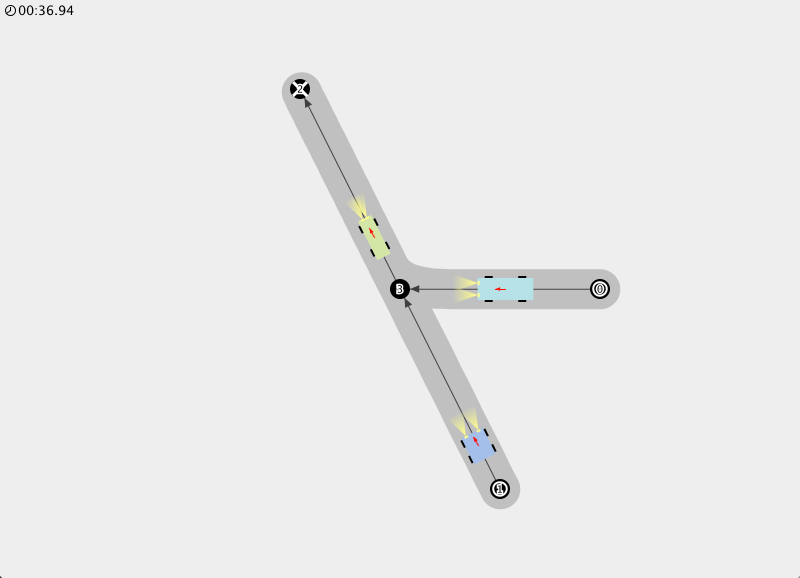
\includegraphics[width=\textwidth]{./img/model_simulationView}
		\caption{Without visible field of view.}
		\label{fig:model:simulation:nofix}
	\end{subfigure}
	\begin{subfigure}{0.49\textwidth}
		\centering
		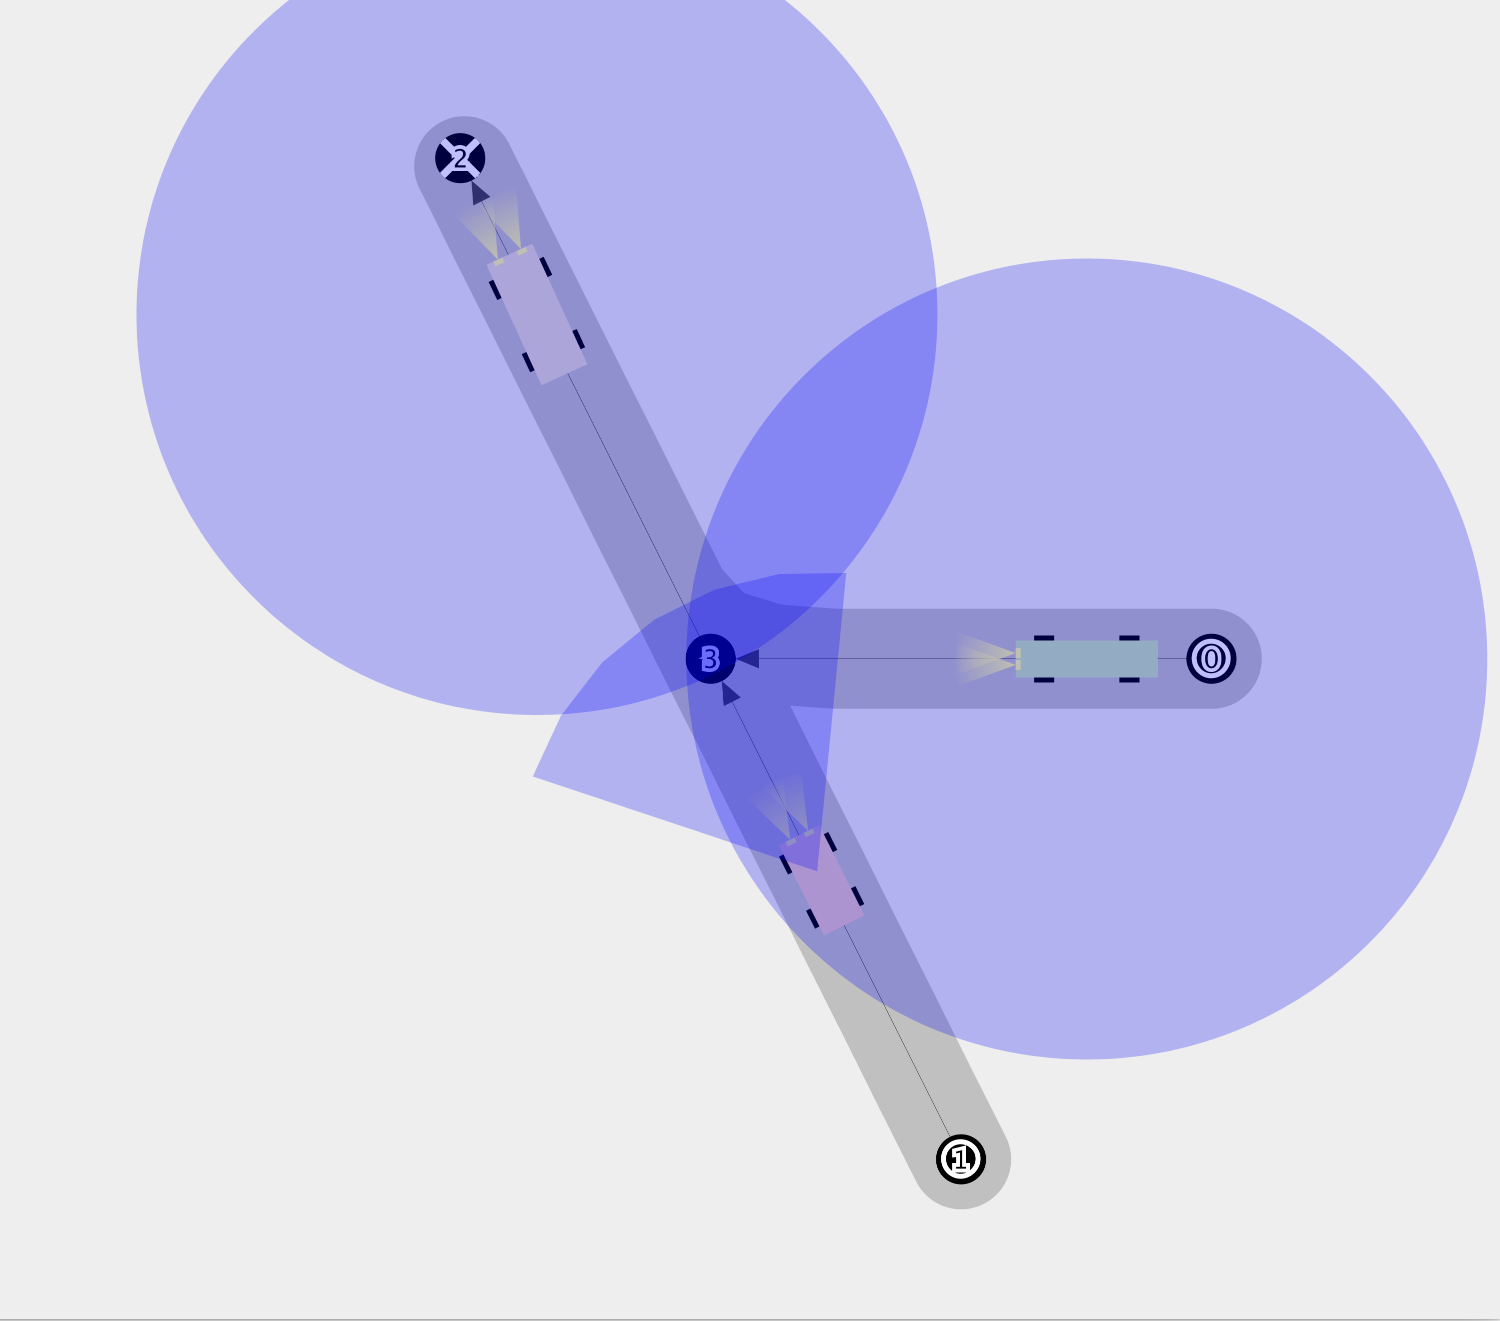
\includegraphics[width=\textwidth]{./img/model_simulationView_fieldOfView}
		\caption{With visible field of view.}
		\label{fig:model:simulation:fix}
	\end{subfigure}	
	\caption{The traffic simulation without \subref{fig:model:simulation:nofix} visible field of view and \subref{fig:model:simulation:fix} with the field of view shown. Dots represent vertices of the graph that we use to represent the road map, vehicles can enter the simulation at the dots with concentric white and black circles, e.g. node 0 or 1 in \subref{fig:model:simulation:nofix}, and can leave it a the black circles with a white cross, e.g. node 2 in \subref{fig:model:simulation:nofix}. Simple black circles represent vertices along a path. The names of the vertices are shown in the circles that represent them. The field of views around the source and sink, shown in \subref{fig:model:simulation:fix} indicate the area that is observed by that vertex.}
	\label{fig:model:simulation}
\end{figure}

\subsubsection{Overview}
\label{subsub:method:model:overview}
%!TEX root = report.tex
\paragraph{Purpose}
\label{par:method:model:overview:purpose}
% \algemeen{A clear, concise and specific formulation of the model’s purpose. This element informs about why you need to build a complex model, and what, in general and in particular, you are going to do with your model.}
The aim of this model is to be able to test whether autonomous vehicles joining regular `human' traffic has influences traffic delays. To do this, we need a simulation in which we have different types of agents, namely autonomous and `human' agents, and a set of roads. In our simulation, we let both types of agents drive over the roads, encounter intersections, and we  measure the delay an number of crashes. By doing this with different ratios of human to autonomous vehicles we can get an idea of when the presences of self-driving cars starts to influence the flow of traffic.

\paragraph{State variables and scales}
\label{par:method:model:overview:state}
This model contains three different hierarchical levels, the car level, driver level and the traffic level. The traffic level contains the roads, and thus all possible paths, and all the vehicles. The car and driver levels consist of all parameters necessary for the functioning of a vehicle. The car level concerns the vehicle itsself, while the driver level implements the driver agent.
\vdbraak{Check that the low-level parameters are still accurate}

\subparagraph{Low-level state variables}
\Cref{tab:par:method:model:overview:state:lowlevel:car} provides an overview of all parameters that influence the behaviour of a car. Since we use a physics engine to realistically model vehicles we need a lot of information on the physical properties of the car. Each car has a driver, this driver can either be autonomous or human. Currently the only difference between human drivers and autonomous drivers is their field of view, however future versions of this system could also include some of the attributes proposed by \citeauthor{paruchuri2002multi}. \jelmer{Physics engine? Explain.}

The \t{path} mentioned in \cref{tab:par:method:model:overview:state:lowlevel:driver} is a set of points in the two dimensional simulation space, the origin of this space lies in the middle of the panels shown in \cref{fig:model:simulation}. 

% The dimensions must be clearly defined for all parameters and variables in the tables.
\jelmer{Target? Who you're trying to hit?}
\jelmer{Er zijn eenheden toegevoegd, aan deze tabel, zou jij kunnen checken of die kloppen.}
\jelmer{Wat is de eenheid van power?}
	\begin{table}
		\centering
		\begin{tabularx}{\textwidth}{>{\ttfamily}llX}
			\toprule
			\normalfont{Parameter}	&Unit & Purpose \\ 
			\midrule
			acceleration 			
				& \si{\meter\per\square\second} 
				& The acceleration of the vehicle, may be negative to indicate breaking.\\ 
			targetBodyAngle 		
				& \si{\radian}
				& The angle at which the target is located, relative to the body of the vehicle. \\ 
			maxSteerAngleDeg 		
				& \si{\radian}
				& The maximum angle the wheels can turn. \\ 
			power 					
				& \si{?}
				& The impulse power of a vehicle. \\ 
			wheelAngleDeg 			
				& \si{\radian}
				& The current angle of the wheel, relative to the body of the vehicle. \\ 
			steeringSpeed 			
				& \si{\meter\per\second}
				& The speed with which a vehicle can turn (the turning radius). \\  
			width 					
				& \si{meter} 
				& The width of the vehicle. \\ 
			length 					
				& \si{meter} 
				& The length of the vehicle. \\ 
			% colour 				& unit & The colour of a vehicle \\ 
			driver 					
				& n.a. 
				& The driver agent. \\ 
			initialPosition 		
				& n.a.
				& The initial position of the agent at the start of the simulation. \\ 
			% bodyFixture 			& unit & The `fixture' of the body of a vehicle, used when viewing other vehicles\\ 
			% visionFixture 		& unit & The `fixture of the vision of the vehicle, describing what a vehicle can see'\\ 
			targetSpeedKMH			
				& \si{\kilo\meter\per\hour}
				& The maximum speed of the agent. \\ 
			\bottomrule
		\end{tabularx}
		\caption{An overview of the parameters that indicate the state of a car.}
		\label{tab:par:method:model:overview:state:lowlevel:car}
	\end{table}

	\begin{table}
		\centering
		\begin{tabularx}{\textwidth}{>{\ttfamily}llX}
			\toprule
			\normalfont{Parameter}	&Unit & Purpose \\ 
			\midrule
			path					
				& n.a. 
				& The path the agent is going to follow. \\ 
			viewLength 			
				& \si{\meter}
				& The radius of the arc that covers the area that is perceived by the driver.\\ 
			actPeriod
				& \si{\milli\second}
				& The period of time to wait before a driver's next \t{act}. 
			\bottomrule
		\end{tabularx}
		\caption{An overview of the parameters that indicate the state of a driver.}
		\label{tab:par:method:model:overview:state:lowlevel:driver}
	\end{table}

	The \t{driver} level, as described in \cref{tab:par:method:model:overview:state:lowlevel:driver}, can be of two different types, `autonomous' or `human'. These are further elaborated on in \cref{sub:method:design}.

	\subparagraph{Higher-level entities}
	The parameters at the simulation level are presented in \cref{tab:par:method:model:overview:state:highlevel:sim}.

	The properties of cars are described in \cref{tab:par:method:model:overview:state:lowlevel:car}. The graph represents the streets, it is input as a connected directed graph with two special types of vertices; sources and sinks. Sources are vertices where cars can enter the simulation, these vertices have no incoming edges, the opposite type of vertex is a sink; vertices without outgoing edges where cars leave the simulation. In terms of traffic a source is the point of departure and a sink is the destination. To determine the \t{path} mentioned in \cref{tab:par:method:model:overview:state:lowlevel:car} we try to find a path from a randomly chosen source to a randomly chosen sink using breadth-first search. The found path is represented as a list of edges, which are then converted to the set of points that make up the \t{path}.
	
	\begin{table}[H]
		\centering
		\begin{tabularx}{\textwidth}{>{\ttfamily}lX}
			\toprule
			\normalfont{Parameter}	& Purpose \\  
			\midrule
			cars 					& A list of the cars in the simulation. \\ 
			streetGraph		 		& A graph representation of the network of streets. \\ 
			\bottomrule
		\end{tabularx}
		\caption{High-level parameters used by the simulation.}
		\label{tab:par:method:model:overview:state:highlevel:sim}
	\end{table}


	\subparagraph{Scales}
	Each time step is \si{33 \milli\second}. This frequent update rate makes the visualisation of the simulation run smoothly, without creating a too large computational stress. Furthermore this small time steps ensures that our simulation approaches the continuous movement of real life vehicles. 
	\jelmer{Klopt dit?}
	At each time step the cars move forward along their \t{paths} one by one. 

\jelmer{Een time horizon (hoe lang de simulatie draait?) kiezen en hier rapporteren.}

	\jelmer{Als er iets in tijdsstappen of planning verandert moet dit geupdate}
	\jelmer{Batch mode in ieder geval noemen.}



\paragraph{Process overview and scheduling}
\label{par:method:model:overview:process}
% \algemeen{Welkeb processen zitten in het model, eventueel met tabel.}


The processes active in the model are \t{steerTowardsPath()}, \t{speedAdjustmentToAvoidCars()} and \t{speedAdjustmentToPreventColission()}. 

The process \t{steerTowardsPath} is the driving of the vehicle in the direction of the target. As a car is added to the simulation it is passed its path, which is defined as multiple discrete points.  A vehicle drives in the direction of the next point on its path, and when it is close enough, drives to its next target, the next point on its path. Eventually the agent will reach its goal, even when it gets diverted by other vehicles along the way.

Both \t{speedAdjustmentToAvoidCars()} and \t{speedAdjustmentToPreventColission()} are used next to the \t{steerTowardsPath} process. The first is used by human drivers, and checks if there is another vehicle or other object in its vicinity and if it is going to hit it given its current driving angle. If a collision seems imminent, the vector describing the direction vector of the vehicle is negated, causing the vehicle to decelerate.

The second is used by autonomous drivers. 
\jelmer{Wat is hier precies het verschil?}


% \algemeen{Bespreek scheduling van processen, welke volgorde uitgevoerd?}
% \algemeen{Are some actions executed in a random order?}
All actions are executed in a fixed order that stays the same for each iteration. At every time step, each agent first checks if there are other cars it could possibly crash into before continuing on towards the target. The agents are updated in the same order in every time step.

% \algemeen{How is time modeled}
% \algemeen{How are actions that happen concurrently IRL executed in the model}
Time is modelled through the time steps in which a vehicle can move. In real life all vehicles move at the same time, whereas the cars in our simulation are updated sequentially. However our small time step ensures that our vehicles approach concurrent actions. 




\subsubsection{Design Concepts}
\label{subsub:method:model:design}
%!TEX root = report.tex
% \algemeen{Bespreek (een subset van) de volgende elementen, niet noodzakelijk in deze volgorde.}
% Ik heb alles waar niet echt iets stond eruit gehaald om het stacato waar Bart het over had eruit te halen.


\paragraph{Agents}
There are a couple differences between human drivers and autonomous agents. Firstly, the view of the human drivers is limited, compared to that of autonomous drivers. Where the autonomous drivers have a circular view in a radius of 12 meters, the human drivers have an arc-shaped view of differing radius. This radius differs per driver. As the drivers are built, they get assigned a \t{viewLength}. This is sampled from a random distribution with a mean of 8 meters and a standard deviation of 2. If the sampled values are below zero, they are clamped to zero, to avoid negative a negative \t{viewLength}. 

Furthermore, human drivers have an \t{actPeriod} of \SI{100}{\milli\second}, which means that \SI{100}{\milli\second} pass between each update step. This causes them to have a slower reaction to the environment than autonomous drivers, which have an \t{actPeriod} of \SI{0}{\milli\second}, which means they always react instantly. 

Lastly, the way drivers react to other vehicles in their neighbourhood differs, this process is discussed in  \cref{par:method:model:overview:process}. 

% \paragraph{Emergence} 
% % \algemeen{Which system-level phenomena truly emerge from individual traits, and which phenomena are merely imposed?}
% There are no system-level phenomena that emerge from individual traits.

% \paragraph{Adaptation} 
% % \algemeen{What adaptive traits do the model individuals have which directly or indirectly can improve their potential fitness, in response to changes in themselves or their environment?}
% The individuals have no adaptive traits.

% \paragraph{Fitness} 
% % \algemeen{Is fitness-seeking modelled explicitly or implicitly? If explicitly, how do individuals calculate fitness?}
% Fitness-seeking is not modelled explicitly. \todo[inline]{Ook niet echt impliciet toch?}

% \paragraph{Prediction} 
% % \algemeen{In estimating future consequences of their decisions, how do individuals predict the future conditions they will experience?}
% Agents are purely reactive, they do not not consider future conditions when deciding on their next action.  

\paragraph{Sensing \& Interaction} 
% \algemeen{What internal and environmental state variables are individuals assumed to sense or “know” and consider in their adaptive decisions?}
Individual vehicles can sense other vehicles and other objects if they are close enough to `see' them. Whether or not a driver is close enough to observe an object depends on its \t{viewLength}. They cannot see into each other's state variables, or those of the simulation. What is actually perceived by an agent depends on its type, self-driving versus human driver, and in the case of the human agent its state. 
\vdbraak{Hoe hangt het van hun state af?}

Although drivers can observe other vehicles and objects they cannot interact with them. Both humans and autonomous vehicles can only see other objects if they appear within that agents' field of view. The field of view of an autonomous driver is larger, and is updated more often, consequently they observe more.

% \paragraph{Interaction} 
% % \algemeen{What kinds of interactions among individuals are assumed?}
% Vehicles can observer other vehicles, but they cannot interact.

% \paragraph{Stochasticity} 
% % \algemeen{Is stochasticicity part of the model? What are the reasons?}
% In this simulation everything is determined, there is no stochasticity.

% \paragraph{Collectives} 
% % \algemeen{Are individuals grouped into some kind of collective, e.g. a social group?}
% There are no collectives in this simulation, all the agents function for themselves.

\paragraph{Observation} 
% \algemeen{How are data collected from the IBM for testing, understanding, and analysing it?}
We measure how long a vehicle takes to get from its point of departure to its destination. The exact measurements  are discussed extensively in \cref{sub:method:design}.




\subsubsection{Details}
\label{subsub:method:model:details}
%!TEX root = report.tex 
\paragraph{Initialisation}
\label{par:method:model:details:initialization}
% \algemeen{How are the environment and the individuals created at the start of a simulation run, i.e. what are the initial values of the state variables? Is initialisation always the same, or was it varied among simulations? Were the initial values chosen arbitrarily or based on data? References to those data should be provided}
The initial variables are partly fixed, partly variable, an overview of all variables relating to cars and their initial values is presented in \cref{tab:par:method:model:details:init:car:value}. The variability is between agents, but not necessarily between simulations. These varying values are chosen arbitrarily for each run of the simulation.
\jelmer{Met java rand? Welke distirbutie samplet die? Als het een linear congruential generator is, is er een maximuum aantal random nummers voor hij herhaalt, hebben wij daar last van? Jelmer: Op het moment is niets willekeurig, behalve de keuze of er een Human driver of een Autonomous Driver wordt geïnstantieerd (middels Random.nextBoolean(), maar dat wordt anders), en wat de bestemming van de nieuwe bestuurder is. (middels Collections.shuffle()) Dit verhaal omzetten in verslag tekst.}


% Initial position
The \t{initialPosition} of a car, i.e. its point of departure, is uniformly and independently sampled from the \t{sources} of the \t{StreetGraph}. 

% Path
The \t{path} of a car starts at the \t{initialPosition} of the car and ends at its destination which is uniformly and independently sampled from the \t{sinks} of the \t{streetGraph}.

% Drivers
The type of \t{driver} is chosen randomly, weighted with the ratio of human driven vehicles to autonomous cars. I.e. if we have nine human drivers for each autonomous car, a driver is nine times as likely to get be driven by a human. 

% Car size
We sample the width and length of a car independently from a uniform distribution. The minimum and the maximum of this distribution are chosen in such a way that cars are no smaller than a 2004 Smart Coupe and no larger than the maximum size of a private car allowed by the Dutch legislation. The exact ranges are presented in \cref{tab:par:method:model:details:init:car:value}.


\begin{table}
	\centering
	\begin{tabularx}{\textwidth}{>{\ttfamily}lX}
		\toprule
		\normalfont{Parameter}	& Value \\  
		\midrule
		acceleration 			
			& \t{NONE} \\ 
		targetBodyAngle 		
			& \SI[mode=text]{0}{\radian} \\ 
		maxSteerAngleDeg 		
			& \SI[mode=text]{40}{\radian} \\ 
		power 					
			& \SI[mode=text]{30}{?}\\ 
		brakePower 		
			& \SI{50}{\meter\per\square\second}\\
		wheelAngleDeg 			
			& \SI[mode=text]{0}{\radian} \\ 
		steeringSpeed 			
			& \SI[mode=text]{5}{\meter\per\second} \\ 
		visionRange 			
			& \SI[mode=text]{8}{\meter} \\ 
		width 					
			& differs per vehicle, in the range \SIrange{1.470}{2.55}{\meter} \\ 
		length 					
			& differs per vehicle, in the range \SIrange{2.540}{12.0}{\meter} \\ 
		driver 					
			& a driver object, determining the agent type \\
		initialPosition 		
			& differs per vehicle. \\ 
		targetSpeedKMH			
			& \SI[mode=text]{0}{\kilo\meter\per\hour} \\ 
		path					
			& differs per vehicle \\ 		
		\bottomrule
	\end{tabularx}
	\caption{An overview of the initialisation of car-owned state parameters.}
	\label{tab:par:method:model:details:init:car:value}
\end{table} 

\jelmer{Hebben we geen vaste init parameters voor de simulatie? En als het random is, waaorm is het ranodm? Random uit welke distributie. Wat is constant, welke waarde heft het dan? Waarom die waarden?}

\jelmer{Wat zijn de simulation variables en kunnen we er dan naar verwijzen of kunnen we een tabelletje toevoegen met deze variablen?}
The simulation variables differ per simulation, and have no fixed initialisation settings.


\paragraph{Input}
\label{par:method:model:details:input}
% \algemeen{The dynamics of many IBMs are driven by some environmental conditions which change over space and time. All these environmental conditions are “input”, i.e. imposed dynamics of certain state variables.}
This simulation requires a graph, sources and sinks in that graph, the locations of vertices in that graph, the human-autonomous ratio and optionally how long the simulation should run. The graph represents the connections between the streets, since we are not interested in graph visualisation one also needs to indicate the location of each vertex in the world space. Vertices can be marked as a source or as a sink, or both, making that vertex a possible starting point or destination for drivers. The human-autonomous ratio indicates how many human drivers we have relative to the number of autonomous cars. It controls the ratio of human cars to autonomous cars that are generated at each source.


\subsection{Experiment Design}
\label{sub:method:design}
%!TEX root = report.tex
To test if autonomous vehicles have an influence on traffic delays and crashes, we run the simulation multiple times, with different autonomous vehicle to human driver ratios.

For each of these runs, we measure the time it takes for each agent to reach its goal, relative to the distance they have to travel from their initial position to the target. Furthermore we keep track of the number of collisions with other agents. 

Using these measurements, we  determine if the number of collisions and the delay time are influenced by the ratio of autonomous agents to the human ones. 

\baakman{Welke statistieken hebben we? Hoe rekenen we ze uit? Waarom zijn ze relevant.}

\baakman{Welke twee grafen (Invoegen, T-splitsing) gebruiken we, waarom deze, plaatjes enzo.}

\baakman{Hoe vaak runnen we, met welke initiele parameters runnen we. Hoe lang runnen we.}

\section{Results}
\label{sec:results}
%!TEX root = report.tex
\todo[inline]{Introductie voor results}

\subsection{Experimental Findings}
\label{sub:results:experimental}
\todo[inline]{Wat hebben en gemeten, plaatjes enzo}

\subsection{Interpretation of Findings}
\label{sub:results:interpretation}
\todo[inline]{Blaat over plaatjes, misschien samentrekken met \cref{sub:results:experimental}.}


\section{Conclusion}
\label{sec:conclusion}
%!TEX root = report.tex
\algemeen{Introductie voor conclusie}

\subsection{Discussion}
\label{sub:conclusion:discussion}
\algemeen{Discussie, conflicteert wat wij gevonden hebben met de resultaten van anderen?}

\subsection{Relevance}
\label{sub:conclusion:relevance}
\algemeen{Waarom is wat wij gevonden hebben relevant, rare plek hiervoor, maar goed.}


\printbibliography

\end{document}